\section{Auswertung}
\label{sec:Auswertung}
Die für den Versuch relevanten Bauteile haben die Werte
\begin{align}
  L & = (\num{16.78 +- 0.09}) \text{mH}	\\
  C & = (\num{2.066 +- 0.006}) \text{nF} \\
  R_1 & = (\num{67.2 +- 0.2}) \Omega \\
  R_2 & = (\num{682 +- 1}) \Omega
  \label{eqn:Bau}
\end{align}
Für den Versuch 3.2 wurde aufgrund eines Defektes des regelbaren Widerstands der Aufbau gewechselt. Die Daten für den Aufgabenteil sind,
\begin{eqnarray}
  L_2 =& (\num{3.53 +- 0.03}) \text{mH}	\\
  C_2 =& (\num{5.08 +- 0.01}) \text{µF}
\end{eqnarray}
\subsection{Zeitabhänigkeit der Amplitude und Dämpfungswiderstand einer Gedämpften Schwingung}
Die durch das Oszilliskop gemessene Spannungspeaks werden mittels einer CWD-Funktion ermittelt und mit deren dazugehörige Zeit in Tabelle \ref{tab:U_C} aufgetragen.
\begin{table}
  \centering
  \begin{tabular}{c c}
    \toprule
    	$U_\text{C}$ / V & $t$ / $10^{-3}$ \, s\\
    \midrule
    \num{52.0 +- 0.1}  	& \num{0.18 +- 0.01}	\\
    \num{48.8 +- 0.1}	& \num{0.54 +- 0.01}	\\
    \num{45.6 +- 0.1}	& \num{0.93 +- 0.01} 	\\
    \num{41.6 +- 0.1}	& \num{1.30 +- 0.01}	\\
    \num{38.4 +- 0.1}	& \num{1.69 +- 0.01}	\\
    \num{36.6 +- 0.1}	& \num{2.09 +- 0.01} 	\\
    \num{34.2 +- 0.1}	& \num{2.46 +- 0.01}	\\
    \num{33.3 +- 0.1} 	& \num{2.82 +- 0.01}	\\
    \num{32.0 +- 0.1} 	& \num{3.20 +- 0.01} 	\\
    \num{31.4 +- 0.1}	& \num{3.59 +- 0.01}	\\
    \num{29.6 +- 0.1}	& \num{3.96 +- 0.01}	\\
    \num{28.8 +- 0.1}	& \num{4.32 +- 0.01} 	\\
    \bottomrule
  \end{tabular}
  \caption{Spannung am Kondensator zur Bestimmung des Abklingverhalten und des Dämpfungswiederstandes.}
  \label{tab:U_C}
\end{table}
Anhand der Daten lassen sich durch eine Fit-Funktion die Koeffizienten der Einhüllenden berechnen, welche in Gleichung \ref{eqn:I} beschrieben ist.
\begin{eqnarray}
  A_0 = ( \num{30.6 +- 0.9} ) \text{V} \\
  f = ( \num{680 +- 60} ) \text{Hz}
  \label{eqn:Koef}
\end{eqnarray}
Die Einhüllende und die Messdaten sind in Abbildung \ref{fig:Osz} dargestellt.
\begin{figure}
  \centering
  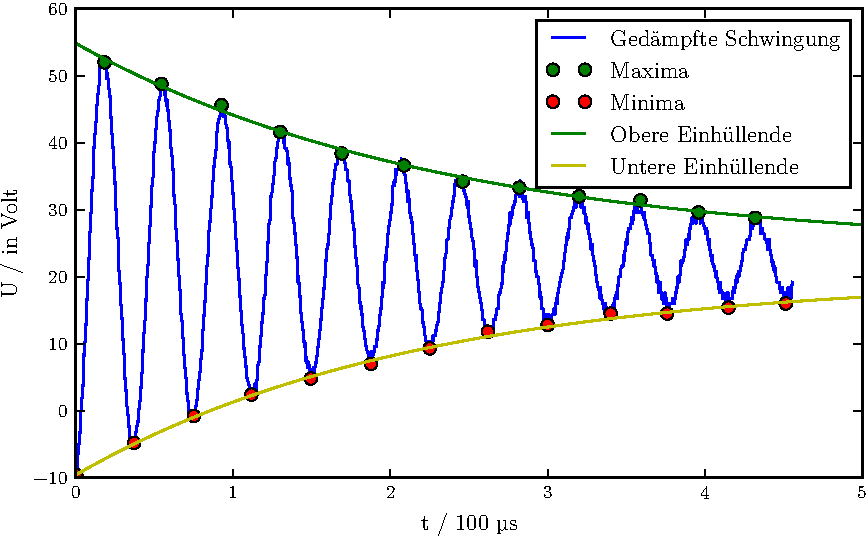
\includegraphics[height=5cm]{plot.pdf}
  \caption{Messdaten mit Einhüllender}
  \label{fig:Osz}
\end{figure}
Nach Formel \ref{eqn:mu} und \ref{eqn:tex} lässt sich der effektive Dämpfungswiderstand sowie die Abklingdauer berechnen.
\begin{eqnarray}
  R_\text{eff} = ( \num{140 +- 10}) \, \Omega \\
  T_\text{ex} = ( \num{230 +- 10}) \cdot 10^{-6} \, \text{s}
  \label{eqn:Reff}
\end{eqnarray}
Der praktisch bestimmte Wert weicht vom errechneten Wert um 75 $\Omega$ ab. Dies lässt sich einerseits dadurch erklären, dass der Innenwiderstand von 50 $\Omega$ nicht berücksichtigt wurde. Andererseits kann es bei der gewählten Frequenz zu Impedanzen der verschiedenen Bauteile gekommen sein. Für die weiteren Aufgaben wird der Widerstand des Generators berücksichtigt.
\subsection{Dämpfungswiderstand des aperiodischen Grenzfalls}
Der im Experiment bestimmte Widerstand, bei dem der Aperiodische Grenzfall eintritt, beträgt
\begin{equation}
  R_\text{Praxis} = 1.25 \, \Omega \ .
  \label{eqn:Rprax}
\end{equation}
Der Theoretische Widerstand wird mittels Formel \ref{eqn:Rap} ausgerechnet und beträgt
\begin{equation}
  R_\text{Theorie} = (\num{2.75 +- 0.23}) \text{\Omega} \ .
  \label{eqn:Rthe}
\end{equation}
Zwischen dem theoretisch und dem praktisch ermittelten Wert ist eine Differenz von \\
1.5 $\Omega$. Mögliche Ursachen für den Fehler sind, die vernachlässigte Impedanz des Aufbaus, als auch die Schwierigkeit den Punkt des Aperiodischen Grenzfalls zu treffen, da keine wesentliche Änderung zu erkennen sind.
\subsection{Frequenzabhängigkeit der Kondensatorspannung eines  Serienresonanzkreis}
In Tabelle \ref{tab:U_c} sind die Spannung am Kondensator und die entsprechenden Frequenzen hinterlegt. Bei den Frequenzen wird ein Ablesefehler von 0.1 V angenommen, da immer auf die erste Stelle nach dem Komma auf- bzw. abgerundet wird.
\begin{table}
  \centering
  \begin{tabular}{c c}
	\toprule
	f / Hz & U / V \\
	\midrule
	9	& \num{5.6 +- 0.1}	\\
	12	& \num{6.4 +- 0.1}	\\
	16	& \num{6.8 +- 0.1}	\\
	23	& \num{7.2 +- 0.1}	\\
	35	& \num{7.2 +- 0.1}	\\
	61	& \num{7.6 +- 0.1}	\\
	162	& \num{7.6 +- 0.1}	\\
	307	& \num{7.6 +- 0.1}	\\
	500	& \num{7.6 +- 0.1}	\\
	905	& \num{7.6 +- 0.1}	\\
	1604	& \num{7.8 +- 0.1}	\\
	2509	& \num{7.8 +- 0.1}	\\
	4025	& \num{7.8 +- 0.1}	\\
	5615	& \num{8.0 +- 0.1}	\\
	8970	& \num{9.0 +- 0.1}	\\
	12030	& \num{10.0 +- 0.1}	\\
	15400	& \num{11.2 +- 0.1}	\\
	17610	& \num{13.0 +- 0.1}	\\
	20000	& \num{15.6 +- 0.1}	\\
	22520	& \num{20.4 +- 0.1}	\\
	24000	& \num{24.8 +- 0.1}	\\
	24490	& \num{26.0 +- 0.1}	\\
	25180	& \num{27.6 +- 0.1}	\\
	25570	& \num{28.0 +- 0.1}	\\
	26300	& \num{28.4 +- 0.1}	\\
	27060	& \num{27.2 +- 0.1}	\\
	27610	& \num{26.0 +- 0.1}	\\
	28100	& \num{24.2 +- 0.1}	\\
	29970	& \num{18.0 +- 0.1}	\\
	32540	& \num{12.4 +- 0.1}	\\
	35660	& \num{8.6 +- 0.1}	\\
	40030 	& \num{5.4 +- 0.1}	\\
	42580 	& \num{4.4 +- 0.1}	\\
	45000	& \num{3.7 +- 0.1}	\\
	50180	& \num{2.7 +- 0.1}	\\
	52430 	& \num{2.4 +- 0.1}	\\
	55010	& \num{2.2 +- 0.1}	\\
	\bottomrule
 	\end{tabular}
  \caption{Frequanzabhängigkeit der Kondensatorspannung}
  \label{tab:U_c}
\end{table}
Anhand derer und der Abbildung \ref{fig:logUc} lässt sich die Güte ablesen.
\begin{figure}
  \centering
  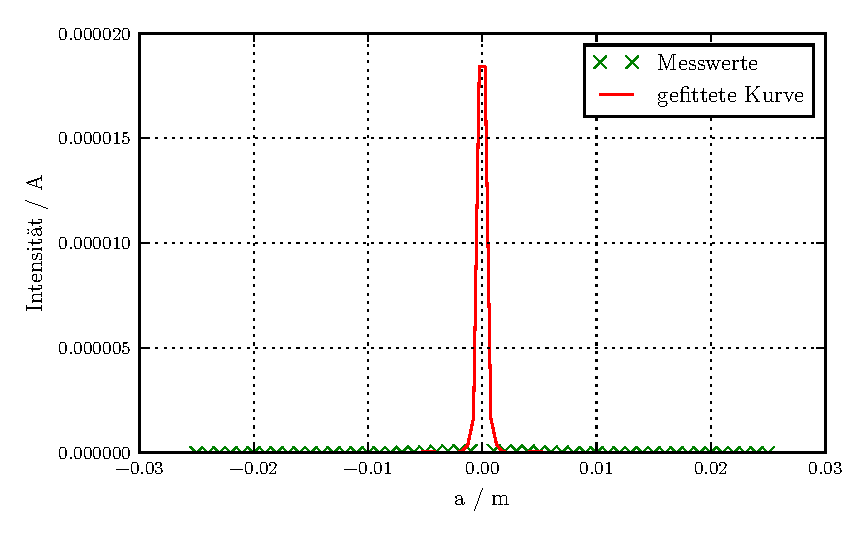
\includegraphics[height=9cm]{plot1.pdf}
  \caption{Halblogaritmisch aufgetragene Kondensatorspannung gegen die Frequenz}
  \label{fig:logUc}
\end{figure}
Er beträgt
\begin{equation}
  q_\text{exp1} = \num{4.30 +- 0.01} \ .
  \label{eqn:qexp}
\end{equation}
Aus Formel \ref{eqn:q} lässt sich der theoretische Wert der Güte berechnen. Sie beträgt
\begin{equation}
  q_\text{theo} = (\num{4.18 +- 0.01})
  \label{eqn:qtheo}
\end{equation}
und ist somit 3 \% größer als der praktisch ermittelte Wert. Mittels eines linearen Plot (siehe Abbildung \ref{fig:fUc}) soll die breite der Resonanzkurve bestimmt werden.
\begin{figure}
  \centering
  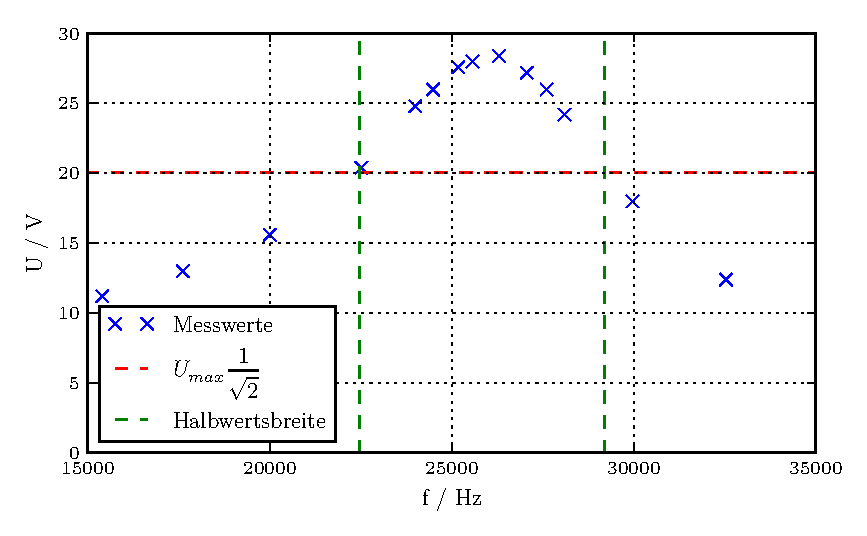
\includegraphics[height=9cm]{plot2.pdf}
  \caption{Frequenzabhängige Kondensatorspannung}
  \label{fig:fUc}
\end{figure}
Durch Ablesen wird die Breite der Resonanzkurve bestimmt welche
\begin{equation}
  v_+ - v_- = 6.72 \, \text{kHz}
\end{equation}
entspricht. Die theoretische breite berechnet sich nach Formel \ref{eqn:qbreite}. Sie beträgt
\begin{equation}
	v_+ - v_- = (\num{6.47 +- 0.04}) \, \text{kHz} \ .
	\label{eqn:nures}
\end{equation}
Die Resonanzfrequenz wird aus dem Graphen abgelesen, bzw der Tabelle entnommen
\begin{equation}
  \nu_\text{res} = (\num{26.30 +- 0.01}) \, \text{kHz} \ .
\end{equation}
Mit Hilfe derer und der Breite der Resonanzkurve lässt sich aus Formel \ref{eqn:qbreite} die praktisch ermittelte Güte berechnen. Daraus folgt eine Güte von
\begin{equation}
  q_\text{exp2} = (\num{3.91 +- 0.08}) \ .
  \label{eqn:qexp2}
\end{equation}
Der experimentell bestimmte Wert weicht vom theoretischen Wert um 6.9 \% ab.
\subsection{Frequenzabhängigkeit der Phase zwischen Erreger- und Kondensatorspannung}
Ziel ist es die Resonanzfrequenz $\nu_\text{res}$ zu bestimmen, sowie die Frequenz $\nu_1$ und $\nu_2$, welche eine Phasenverschiebung von $\frac{\pi}{4}$ und $\frac{3 \pi}{4}$ ergeben. Die Phasenverschiebung zu den entsprechenden Frequenzen sind in Tabelle \ref{tab:phi} aufgetragen und in Abbildung \ref{fig:logphi} in einem halblogarithmischen Plot dargestellt.
\begin{table}
  \centering
  \begin{tabular}{c c}
	\toprule
	$f$ / Hz & $\Phi$ / rad \\
	\midrule
	9   	& \num{0.00 +- 0.02} \\
	12  	& \num{0.00 +- 0.02} \\
	16  	& \num{0.00 +- 0.02} \\
	23  	& \num{0.00 +- 0.02} \\
	35  	& \num{0.00 +- 0.02} \\
	61  	& \num{0.00 +- 0.02} \\
	162 	& \num{0.00 +- 0.02} \\
	307	  & \num{0.00 +- 0.02} \\
	500 	& \num{0.00 +- 0.02} \\
	905 	& \num{0.00 +- 0.02} \\
	1604 	& \num{0.00 +- 0.02} \\
	2509 	& \num{0.00 +- 0.02} \\
	4025 	& \num{0.00 +- 0.02} \\
	5615 	& \num{0.00 +- 0.02} \\
	8970 	& \num{0.00 +- 0.02} \\
	12030	& \num{0.12 +- 0.02} \\
	15400 	& \num{0.27 +- 0.02} \\
	17610 	& \num{0.33 +- 0.02} \\
	20000 	& \num{0.42 +- 0.02} \\
	22520 	& \num{0.62 +- 0.02} \\
	24000 	& \num{0.87 +- 0.02} \\
	24490 	& \num{0.95 +- 0.02} \\
	25180 	& \num{1.20 +- 0.02} \\
	25570 	& \num{1.25 +- 0.02} \\
	26300 	& \num{1.45 +- 0.02} \\
	27060 	& \num{1.70 +- 0.02} \\
	27610 	& \num{1.97 +- 0.02} \\
	28100 	& \num{1.90 +- 0.02} \\
	29970 	& \num{2.37 +- 0.02} \\
	32540 	& \num{2.69 +- 0.02} \\
	35660 	& \num{2.82 +- 0.02} \\
	40030 	& \num{3.16 +- 0.02} \\
	42580 	& \num{2.88 +- 0.02} \\
	45000 	& \num{2.88 +- 0.02} \\
	50180 	& \num{2.96 +- 0.02} \\
	52430 	& \num{3.09 +- 0.02} \\
	55010 	& \num{3.11 +- 0.02} \\
  \end{tabular}
  \caption{Phasenverschiebung in Abhängigkeit der Frequenz}
  \label{tab:phi}
\end{table}
\begin{figure}
  \centering
  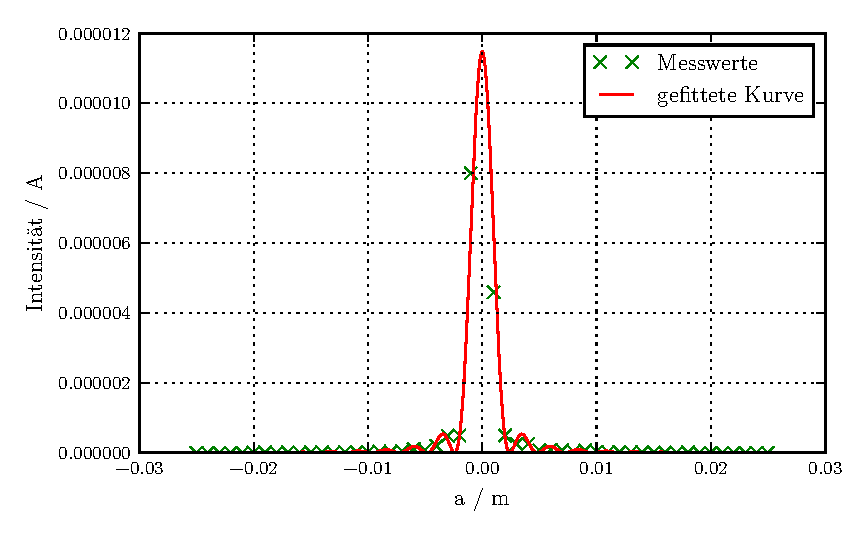
\includegraphics[height=9cm]{plot3.pdf}
  \caption{Phasenverschiebung zwischen Erreger- und Kondensatorspannung}
  \label{fig:logphi}
\end{figure}
Dem Plot wird entnommen, dass erst ab einer Frequenz von ca. 10 kHz eine Phasenverschiebung zu bemerken ist. Um die Resonanz besser bestimmten zu können werden die Werte in Abbildung \ref{fig:Phi} linear um die Resonanzfrequenz dargestellt.
\begin{figure}
  \centering
  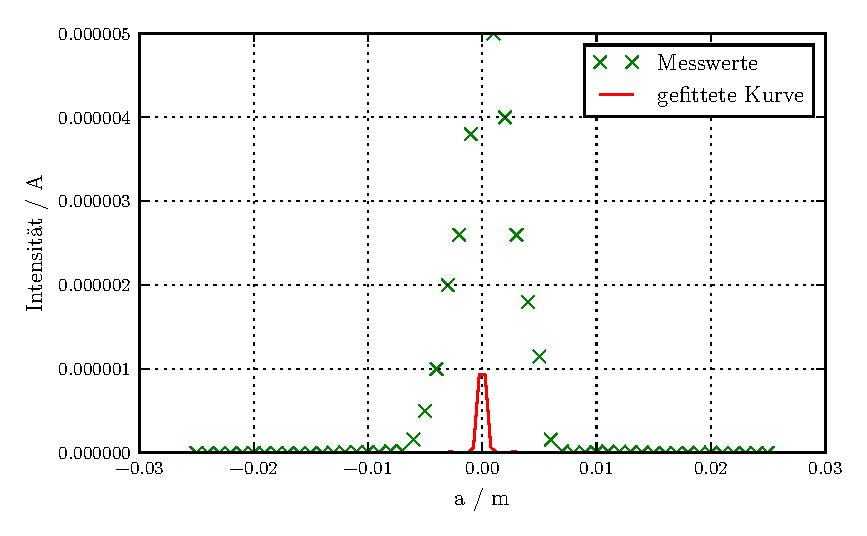
\includegraphics[height=9cm]{plot4.pdf}
  \caption{Phasenverschiebung zwischen Erreger- und Kondensatorspannung}
  \label{fig:Phi}
\end{figure}
Mittels eines Fit werden die Messwerte durch eine Funktion der Form
\begin{eqnarray}
  \Phi (\nu)  =& \arctan(\nu \cdot a + b) + c \\
  \label{pfit}
  a =& (\num{3.4 +- 0.1}) \cdot 10^{-4}\\
  b =& (\num{-9.1 +- 0.5})\\
  c =& (\num{1.50 +- 0.02})\\
\end{eqnarray}
approximiert. Anhand des Fits lassen sich die Frequenzen zu den Phasenverschiebung von $\frac{\pi}{4}$ und $\frac{3 \pi}{4}$ durch umstellen berechnen. Die theoretische Resonanzfrequenz berechnet sich aus Formel \ref{eqn:wres} und die Frequenzen $\nu_1$ und $\nu_2$ aus der Formel \ref{eqn:w12}. In Gleichung \ref{eqn:res} wird die theoretisch ermittelte mit der praktisch ermittelten Güte verglichen und der Fehler berechnet.
\begin{eqnarray}
  \nu_\text{res,exp} =&  (\num{26 +- 2}) \, \text{kHz}			\\
  \nu_\text{res,theo} =& (\num{26.58 +- 0.08}) \, \text{kHz} \\
  \text{Abweichung} =& 0.23 \%
  \label{eqn:res}
\end{eqnarray}
Analog wird mit den Werten für $\nu_1$ und $\nu_2$ vorgangen.
\begin{eqnarray}
  \nu_\text{1,exp} =&  (\num{23 +- 2}) \, \text{kHz}                 \\
  \nu_\text{1,theo} =& (\num{23.78 +- 0.07}) \, \text{kHz} \\
  \text{Abweichung} =& 3 \%
\end{eqnarray}
\begin{eqnarray}
  \nu_\text{2,exp} =&  (\num{29 +- 2}) \, \text{kHz}                 \\
  \nu_\text{2,theo} =& (\num{30.7 +- 0.1}) \, \text{kHz} \\
  \text{Abweichung} =& 4 \%
\end{eqnarray}
Die Güte berechnet sich aus Formel \ref{eqn:qbreite} und beträgt
\begin{equation}
  q_\text{exp3} = \{ref{4 +- 2}  \ .
  \label{eqn:q3}
\end{equation}
Dies entspricht einer prozentualen Abweichung von 4.5 \% vom Theoriewert.
